\chapter{Operations on $t$\hyp{}structures}\label{chap:operat}
\thispagestyle{empty}
In this chapter we collect several examples of operations on the set of $t$\hyp{}structures on a fixed  $\infty$\hyp{}category $\CC$, and functions between classes of $t$\hyp{}structures on different categories. 

From a formal point of view, this amounts to a study of  closure properties of the $\infty$\hyp{}category whose objects are categories with $t$\hyp{}structure, $(\CC,\tee_\CC)$. These objects will be called \emph{$t$\hyp{}structured categories} and they will be collected in the $\infty$\hyp{}category $\Cat_\tee$. There is an obvious forgetful functor $U\colon \Cat_\tee \to \Cat_\text{st}$, which has adjoints on both sides; again from a formal point of view, some of the results below amount to a(n easy) series of verification that $U$ has some nice properties.\index{Category!--- with $t$\hyp{}structure}

As it has been observed in \achap \refbf{chap:hearts} the poset $\ts(\CC)$ of $t$\hyp{}structures on $\CC$ has a fairly rich structure: it is a partially ordered set, with a canonical action of the group of integers given by the shift functor (see \refbf{slicing}); it is often the case that nice properties on $\CC$ turn $\ts(\CC)$ into a nicer poset: as we will see in \S\refbf{tens.of.tee}, the class $\ts(\sp)$ of $t$\hyp{}structures on the $\infty$\hyp{}category of \emph{spectra} becomes a monoid under the operation described there.

Among the most natural operations on categories there is their product: it is easy to show that given stable $\infty$\hyp{}categories $\CC,\D$ the product $\CC\times \D$ is again stable;\footnote{There are at least two ways to prove this; directly, or appealing to \cite[\textbf{1.1.4.2}]{LurieHA}.} from a torsio\hyp{}centric perspective, it is then natural to give the following
\index{t-structure@$t$\hyp{}structure!product of ---s}
\begin{definition}[product $t$\hyp{}structure]\label{product.of.fact}
Given stable $\infty$\hyp{}categories $\CC,\D$ the \emph{product} $t$\hyp{}structure $\tee_\CC\times \tee_\D$ on the product category $\CC\times \D$ is defined to be the product (defined in \refbf{prod.of.fact}) of the factorization systems $\fF(\tee_\CC)\times \fF(\tee_\D)$ (the notation is the same of \athm \refbf{thm:rosetta}).
\end{definition}
\index{t-structure@$t$\hyp{}structure!co\fshyp{}induction of ---s}
\section{Basic constructions.}
% \epigraph{MANCA!}{}
\begin{definition}[induced $t$\hyp{}structure]
Let $\cate{B}\subseteq \CC$ be a stable sub\hyp{}$\infty$\hyp{}category; let $0/\EE|_\cate{B} = 0/\EE\cap \cate{B}, \MM/0|_\cate{B} = \MM/0\cap \cate{B}$ considered as full subcategories; then if the truncation and cotruncation functors $S_\CC,R_\CC$ restrict to functors $\cate{B}\to 0/\EE|_\cate{B}, \MM/0|_\cate{B}$ the category $\cate{B}$ inherits a $t$\hyp{}structure called the \emph{restricted} or \emph{induced} $t$\hyp{}structure $\tee|_\cate{B}$.
\end{definition}
The proof is straightforward as restricting the co\fshyp{}truncation functors is a sufficient condition to ensure the existence of $\tee|_\cate{B}$. Note that in principle this is a weaker condition than having an induced normal torsion theory on $\cate{B}$, but that the latter stronger condition is the most natural to expect in concrete situations, as the following example shows.
\begin{example}
Let $F\colon (\CC,\tee_\CC) \to (\D, \tee_\D)$ be a $t$\hyp{}exact functor (\adef \refbf{t.exact.func}); the \emph{fiber} of $F$ is defined by the pullback square (taken in the $(\infty,2)$\hyp{}category of stable $\infty$\hyp{}categories)
\[
\begin{kD}
\lattice[mesh]{
	\obj (B):\fib(F); & \obj \CC; \\
	\obj (0):\cate{0}; & \obj (D):\D.; \\
};
\mor B -> CC F:-> D <- 0 <- B;
\pullback{B}{D};
\end{kD}
\]
In other words, $\fib(F)$ is the full subcategory on all those $X\in\CC$ such that $FX\cong 0$. The fiber of $F$ inherits the induced $t$\hyp{}structure, given that the factor (\adef \refbf{space.of.facts}) of the $\fF(\tee_\CC)$\hyp{}factorization of a morphism in $\fib(F)$ lies again in $\fib(F)$.
\end{example}
\begin{definition}[co\hyp{}induced $t$\hyp{}structure]
The \emph{Verdier quotient} $\CC/\cate{B}$ of $\CC$ by a (non necessarily thick) sub\hyp{}$\infty$\hyp{}category $\cate{B}$ is defined to be the universal functor out of $\CC$ sending objects $\cate{B}$ to zero (or, equivalently, formally inverting those morphisms whose cofiber is in $\cate B$).

In the stable setting, the quotient $\CC/\cate{B}$ is again a stable $\infty$\hyp{}category.\footnote{It is the main aim of \cite{} to show that this quotient operation enjoys the universal property of the cofiber $\varinjlim(0\leftarrow \cate{B}\to \CC)$ in the ($\infty$\hyp{})category of stable $\infty$\hyp{}categories.}

Under suitable assumptions, the quotient $\CC/\cate{B}$ acquires a $t$\hyp{}structure defined by \cite[\aprop \textbf{1.4.4.11}]{LurieHA}: in the same notation as above, suppose $\cate{B},\CC$ are presentable and $i\colon \cate{B}\to \CC$ is a fully faithful inclusion. Suppose $\tee\in\ts(\CC)$ is a presentable $t$\hyp{}structure.

The quotient functor $q\colon \CC \to \CC/\cate{B}$ generates the left class of a $t$\hyp{}structure $(q(\CC_{\ge 0}), q(\CC_{\ge 0})^\perp)$ on $\CC/\cate{B}$ by \cite[\aprop \textbf{1.4.4.11}]{LurieHA}.
\end{definition}
\begin{remark}
Here we offer a counterexample \cite{237502} showing that there are cases where this procedure can't induce a $t$\hyp{}structure on the quotient: suppose that there is an exact and fully faithful inclusion $\cate{B}\rightarrow \CC$ of categories with $t$\hyp{}structure.

From this we deduce an exact functor between hearts $\cate{B}^\heart\rightarrow \CC^\heart$ on hearts; notice that $\cate{B}^\heart$ is a so\hyp{}called \emph{weak Serre} subcategory of $\CC^\heart$ (it is closed under extensions, kernels, and cokernels). In order for there to be a $t$\hyp{}structure on $\CC/\cate{B}$ such that $q\colon \CC\rightarrow \CC/\cate{B}$ is exact, $\cate{B}^\heart$ must be Serre, \ie also closed under subobjects.

A concrete case where this doesn't happen is as follows. Suppose that $R$ is a coherent commutative ring. This means that every finitely generated ideal of $R$ is finitely presented, and it has the consequence that the category of finitely presented $R$\hyp{}modules is abelian. Let's call this category $\smallcap{Coh}(R)$ and view it as a full subcategory of $\cate{Mod}(R)$. We can consider $D^b_{\smallcap{Coh}(R)}(\cate{Mod}(R))\subseteq D^b(\cate{Mod}(R))$, where the category consists of bounded complexes of $R$\hyp{}modules with homology modules in $\smallcap{Coh}(R)$. There are clearly bounded $t$\hyp{}structures on these. However, if $R$ is not noetherian, then the heart of the first, namely $\smallcap{Coh}(R)$, will not be Serre inside the heart of the second, namely $\cate{Mod}(R)$.
\end{remark}
\section{The poset of $t$\hyp{}structures.}\index{t-structure@$t$\hyp{}structure!poset of ---s}
Studying the order\hyp{}theoretic properties of the set $\ts(\CC)$ should be a natural step towards the classification of $t$\hyp{}structures on $\CC$.

It is natural, then, to ask whether $\ts(\CC)$ admits finite joins and meets: a natural way to define these operations on $\tee_1 = (\CC_{\ge 0}^{(1)}, \CC_{<0}^{(1)})$ and $\tee_2=(\CC_{\ge 0}^{(2)}, \CC_{<0}^{(2)})$ intersects respectively the aisle and the coaisle, setting
\begin{align}
\tee_1\cap \tee_2 &= \Big(\CC_{\ge 0}^{(1)}\cap \CC_{\ge 0}^{(2)}, perp.\Big)\label{naivemeet}\\
\tee_1\cup \tee_2 &= \Big(perp.', \CC_{< 0}^{(1)}\cap \CC_{< 0}^{(2)}\Big)\label{naivejoin}
\end{align}
where $perp.$ is a shorthand for $\big(\CC_{\ge 0}^{(1)}\cap \CC_{\ge 0}^{(2)}\big)^\perp$, and $perp.'$ is a shorthand for $\prescript{\perp}{}{\big(\CC_{< 0}^{(1)}\cap \CC_{< 0}^{(2)}\big)}$. These are called the \emph{na\"{\i}ve join} and \emph{na\"{\i}ve meet} respectively.

It is often the case, however, that the na\"{\i}ve join and meet operations in $\ts(\CC)$ do not coincide with the ``abstract'' operations on the same set, definable via universal properties: \cite[\S\textbf{1.2}]{bondal2013operations} gives an example where the intersection $\CC_{\ge 0}^{(1)}\cap \CC_{\ge 0}^{(2)}$, seen as a subcategory of $\CC$, can't be coreflective.

Because of this, $\ts(\CC)$ seems to be rather poorly\hyp{}behaved from the order\hyp{}theoretic point of view. In fact, it is also possible to show that binary meet and join, when defined, do not distribute over each other.

It is however possible to give conditions on $\tee_1,\tee_2$ ensuring that the expected operations exist and behave nicely: this is the main aim of \cite{bondal2013operations}, which we now follow closely: the final aim is to show that $\ts(\CC)$ is a \emph{set with consistencies} \index{Conset} (or a \emph{conset} for short), \ie a partially ordered set where the domain of definition for joins and meets is determined by ``consistency conditions'' on the arguments, and where ``partial distributivity laws'' (\cite[\S 2.1]{bondal2013operations}) hold.

Obviously, we state the consistency conditions for two $t$\hyp{}structures on $\CC$ in terms of the corresponding normal torsion theories.
\begin{definition}[Upper and lower consistency]
Let $\fF_1, \fF_2$ be two normal torsion theories on the stable $\infty$\hyp{}category $\CC$ ($\fF_i = (\EE_i,\MM_i)$), and let $(S_i, R_i)$ be the pair coreflection\fshyp{}reflection of $\fF_i$. Then $\fF_1, \fF_2$ are \emph{lower consistent} (resp., \emph{upper consistent}) if $S_1(0/\EE_2)\subseteq 0/\EE_2$ (resp., $R_2(\MM_1/0)\subseteq \MM_1/0$).

``Being upper\fshyp{}lower consistent'' are symmetric binary relations on the set $\ts(\CC)$ denoted respectively $\upcons$ and $\lowcons$.\index{.upcons-lowcons@$\upcons$ and $\lowcons$} Two normal torsion theories $\fF_1,\fF_2$ which are both lower and upper consistent are simply called \emph{consistent} and this relation is denoted $\fF_1\cons \fF_2$.
\end{definition}
\begin{proposition}
Let $\tee_1,\tee_2$ be a lower consistent pair of $t$\hyp{}structures on $\CC$. Then the naive intersection (\refbf{naivemeet}) is the meet $\tee_1\land \tee_2$. Dually, let $\tee_1,\tee_2$ be upper consistent; then the naive union (\refbf{naivejoin}) is the join $\tee_1\vee\tee_2$.
\end{proposition}
\begin{remark}
It is easy to show that if $\tee_0\preceq \tee_1$ then $\tee_0\cons\tee_1$, and the join\fshyp{}meet of the two is $\tee_1$\fshyp{}$\tee_0$.
\end{remark}
\begin{remark}
\cite[\aprop \textbf{5}, \textbf{6}]{bondal2013operations} prove that lower or upper consistency is a sufficient condition ensuring that the intersection or union of $t$\hyp{}structures exists: given an $n$\hyp{}tuple $\{\tee_1,\dots, \tee_n\}$ of $t$\hyp{}structures
\begin{itemize}
\item if $\tee_i\lowcons \tee_j$ for each $i<j$, then the na\"{\i}ve intersection $\tee_1\cap \dots\cap \tee_n$ is well\hyp{}defined (it coincides with the abstract one) and associative;
\item if $\tee_i\upcons \tee_j$ for each $i<j$, then the na\"{\i}ve union $\tee_1\cup \dots\cup \tee_n$ is well\hyp{}defined (it coincides with the abstract one) and associative.
\end{itemize}
Consistency conditions on $t$\hyp{}structures also ensure that the meet and join distribute over each other:
\begin{itemize}
\item if $\tee_1\upcons \tee_2$, $\tee_1\upcons \tee_3$, and $\tee_2\lowcons \tee_3$ then $\tee_1\upcons (\tee_2\cap \tee_3)$;
\item if $\tee_1\lowcons \tee_3$, $\tee_2\lowcons \tee_3$, and $\tee_1\upcons \tee_2$ then $(\tee_1\cup \tee_2)\lowcons \tee_3$.
\end{itemize}
\end{remark}
The structure so determined is a \emph{set with consistencies}, defined in \cite[\S\textbf{2.1}]{bondal2013operations}.
\section{Tensor product of $t$\hyp{}structures.}\label{tens.of.tee}
\index{t-structure@$t$\hyp{}structure!tensor of ---s}
\epigraph{All God's children are not beautiful. Most of God's children are, in fact, barely presentable.}{F\@. Leibowitz}
Let $\CC,\D$ be two presentable $\infty$\hyp{}categories (\cite[\achap \textbf{5}]{HTT}); then, for each presentable $\infty$\hyp{}category $\A$ we consider the category $\text{Bil}(\CC,\D;\A)$ of functors $F\colon \CC\times \D \to \A$ such that each restriction $F(-,D)$ and $F(C,-)$ is cocontinuous. These functors are called \emph{bilinear}.

It turns out (\cite{Gro,LurieHA,LurieSAG}) that the functor $\A\mapsto \text{Bil}(\CC,\D;\A)$ functor is representable for each pair of categories $\CC,\D$ and represented by an object $\CC\otimes \D$ called the \emph{tensor product} of the two presentable $\infty$\hyp{}categories $\CC,\D$ (the analogy with the tensor product of vector spaces is evident).\index{.CotimesD@$\CC\otimes\D$}\index{.Qcat(Cop,D)@$\QCat(\CC^\text{op},\D)_R$}

Although we are only interested in the case where the categories involved are stable (and then their tensor product is again stable), this condition plays no r\^ole in the proof of
\begin{lemma}\label{tensor.is.repre}
The $\infty$\hyp{}category $\CC\otimes \D$ such that
\[
\text{Bil}(\CC,\D;\A)\cong \QCat(\CC\otimes\D, \A)
\]
is equivalent to $\QCat(\CC^\text{op},\D)_R$, the sub\hyp{}$\infty$\hyp{}category of functors $F\colon \CC^\text{op}\to \D$ that commute with limits. 
\end{lemma}
\begin{proof}
It is a long and formal argument based on universal properties.
\end{proof}
\begin{proposition}
If $\CC,\D$ are \emph{stable} and presentable, the category $\CC\otimes \D$ is stable and presentable as well, and we have that $\CC\otimes \D \cong \QCat(\CC^\text{op},\D)_R$.
\end{proposition}
\begin{proof}
A slick proof that $\QCat(\CC^\text{op},\D)_R$ is presentable is in \cite[p\@. 68]{Gro}; showing that this category is also stable is a matter of unwinding definitions, or follows from our Lemma \refbf{magicstable}. 
\end{proof}
A natural question arises: does the tensor operation lifts from $\Cat_\text{st}$ to $\Cat_\tee$? In other words, given $t$\hyp{}structures $\tee_\CC$ and $\tee_\D$ on categories $\CC,\D$, how can we endow $\CC\otimes \D$ with a $t$\hyp{}structure $\tee_\CC \otimes \tee_\D$ such that the following reasonable properties are satisfied?
\begin{itemize}
\item The operation $(\tee_\CC, \tee_\D)\mapsto \tee_\CC \otimes \tee_\D$ is ``associative'', namely the two $t$\hyp{}structures $(\tee_0\otimes \tee_1)\otimes \tee_2$ and $\tee_0 \otimes (\tee_1\otimes \tee_2)$ correspond to each other via the equivalence $\CC_0\otimes (\CC_1\otimes \CC_2)\cong (\CC_0\otimes \CC_1)\otimes \CC_2$, and ``commutative'', namely the $t$\hyp{}structures $\tee_0\otimes \tee_1$ and $\tee_1\otimes \tee_0$ correspond to each other via the equivalence $\CC_0\otimes \CC_1\cong \CC_1\otimes \CC_0$; moreover, $\otimes \colon \ts(\CC_0)\otimes \ts(\CC_1) \to \ts(\CC_0\otimes \CC_1)$ is compatible with shifts, in the sense that
\[
\tee_0[n]\otimes \tee_0[m] = (\tee_0 \otimes \tee_1)[n+m]
\]
for each $n,m\in\mathbb{Z}$.
\item The canonical $t$\hyp{}structure $\tee_\sp$ on the category $\sp$ of spectra is the unit for this monoidal composition, namely $\tee_\sp\otimes \tee\in \ts(\sp\otimes \CC)$ and $\tee\otimes \tee_\sp\in\ts(\CC\otimes \sp)$ both correspond to $\tee \in\ts(\CC)$ under the equivalence $\sp\otimes \CC \cong \CC \cong \CC \otimes \sp$;
\item Tensoring with a fixed $\tee\in\ts(\sp)$ gives an endofunction $\tee\otimes \tee_\CC$ of $\ts(\CC)$, when composed with the equivalence $\ts(\sp\otimes \CC)\cong \ts(\CC)$; more precisely, there is an action $\ts(\sp) \times \ts(\CC) \to \ts(\CC)$, that becomes a monoid operation when $\CC =\sp$.
\end{itemize}
It turns out that this problem has a natural reformulation in terms of normal torsion theories, as it is rather easy to use the presentability of the categories involved to invoke the small object argument and produce a factorization system on $\CC\otimes \D$. In particular, we rephrase the question in the following form:
\begin{quote}
Given two normal torsion theories $\fF_\CC$ and $\fF_\D$ on two presentable, stable $\infty$\hyp{}categories $\CC,\D$, define a new normal torsion theory $\fF_\CC\otimes \fF_\D$ on $\CC\otimes \D$, having the ``nice'' properties above.
\end{quote}
To solve this problem, consider first of all the explicit formula in Lemma \refbf{tensor.is.repre} which defines $\CC\otimes \D$: as always, solving this universal problem gives a unique map $\CC\times \D \to \CC\otimes \D$, which is the unique bilinear functor corresponding to $1_{\CC\otimes \D}$; this will be called the \emph{canonical tensor}
\[
\otimes \colon \CC \times \D \to \CC\otimes \D
\]
This problem can be divided into several steps: first of all we want to induce a factorization system on $\CC\otimes\D$ starting from factorization systems on the factors $\CC, \D$. Next we want to see that this induced factorization system still has all the good features enjoyed by $\fF_\CC$ and $\fF_\D$; the canonical tensor, together with its domain and codomain, plays an essential r\^ole here (notice that, again, stability is not a necessary condition, but only the most important case of interest for the present discussion):
\begin{itemize}
\item Consider the product of categories $\CC\times \D$ and the product $t$\hyp{}structure $\fF_\CC\times \fF_\D$ (\adef \refbf{product.of.fact}) on this category; by \refbf{uniquely.determines.class} the left class $\EE\times \EE'$ of this factorization system uniquely determines $\MM\times \MM'$ as its right orthogonal, so we will consider only $\EE\times \EE'$ in the following to simplify the discussion.
\item Consider the image $\EE \otimes \EE'$ of $\EE\times \EE'$ via the canonical tensor $\otimes$; this, as a class of morphisms in $\CC \otimes \D$ has a right orthogonal $(\EE \otimes \EE')^\perp$;
\item \index{.F1tensorF2@$\fF_\CC\otimes\fF_\D$} The small object argument (\cite{Joyalcatlab} or \cite{Dwyer1995}) applied to the class $\EE\otimes \EE'$ entails that the pair
\[
(\mcal{L}, \mcal{R}) = \big(\textsf{s}(\EE \otimes \EE'), (\EE \otimes \EE')^\perp\big)
\]
where $\textsf{s}(-)$ is the \emph{saturation} operator defined in \refbf{def:satusatu}, forms a factorization system on $\CC\otimes \D$.
\end{itemize}
\section{Tilting of $t$\hyp{}structures.}
\index{t-structure@$t$\hyp{}structure!tilting of ---s}
\epigraph{Quando si vuole uccidere un uomo bisogna colpirlo al cuore, e un Winchester è l'arma più adatta.}{Ramón Rojo}
Let us first recall (\adef \refbf{df:abelinfty}) that an abelian $\infty$\hyp{}category is an $\infty$\hyp{}category with biproducts, kernels and cokernels, and image\hyp{}factorization which is in addition \emph{homotopically discrete}.

It is not surprising that the language of abelian $\infty$\hyp{}categories is rich enough to interpret the notion of normal torsion theory:\footnote{This is the context where historically torsion theories were introduced \cite{dickson1966torsion}; in some sense, stable categories are ontologically more primitive since ``all'' abelian categories arise as hearts of suitable $t$\hyp{}structures.} to be more precise, we can define a (normal) torsion theory on an abelian $\infty$\hyp{}category $\A$ in a similar fashion of \adef \refbf{normal}, paying attention to the fact that the stable setting endows the definition with several useful autodualities (like \refbf{slex.simple.normal}) false in the abelian setting.

Start with the following example: let $\CC = \cate{D}(\A)$ be the derived $\infty$\hyp{}category of an abelian category $\A$; it is interesting to ask which (factorization functors of) normal torsion theories $\tee_\CC$ on $\D(\A)$ factor through $\A = \D(\A)^\heart \subset \D(\A)$; this means that
\begin{enumerate}
\item we have (mild) co\fshyp{}completeness conditions on $\A$ (\ie the existence in $\A$ of the co\fshyp{}limits involved in \refbf{rmk:how.to.fact});
\item the reflection $R$ and coreflection $S$ of $\tee_\CC$ factor as follows:
\[
\xymatrix{
	\CC^\heart \ar[rr]^{S|_{\CC^\heart}}\ar@{.>}[dr]_{\hat S} && 0/ \EE \\
	 & 0/\EE \cap \CC^\heart \ar[ur]
}\qquad
\xymatrix{
	\CC^\heart \ar[rr]^{R|_{\CC^\heart}}\ar@{.>}[dr]_{\hat R}  && \MM/0 \\
	 & \MM/0 \cap \CC^\heart \ar[ur]
}
\]
\end{enumerate} 
This informal definition is needed to cope with a torsio\hyp{}centric reformulation of \emph{tilting theory}. Our aim here is not to delve into the details of such an intricate and vast topic, but only to skim the surface of it: indeed, 
at the level of generality we are interested in, \emph{tilting} of a $t$\hyp{}structure $\tee$ is a device to produce another $t$\hyp{}structure out of $\tee$ and a (normal) torsion theory on the heart $\CC^{\heart, \tee}$; the $t$\hyp{}structure on $\CC$ are acted by (normal) torsion theories on their hearts.
\begin{definition}
Let $\CC$ be a stable $\infty$\hyp{}category, $\fF = (\EE, \MM)$ a normal torsion theory on $\CC$ and $\mathbb{T} = (\mcal{X}, \mcal{Y})$ a (normal?) torsion theory on the heart $\CC^{\heart, \tee}$. We define the two classes
\begin{align}
\EE \tilt \mcal{X} &= \{f\in \hom(\CC)\mid f\in \EE [-1],\; h_\tee(f)\in \mcal{X}\}\notag\\
\MM \tilt \mcal{Y} &= \{g\in \hom(\CC)\mid g\in \MM [1], \; h_\tee(g)\in \mcal{Y}\},\footnotemark
\end{align}
\footnotetext{The symbol $\tilt$ (pron. \emph{retort}) recalls the alchemical token for an alembic; here the term hints at the double meaning of the word retort.}
where $h_\tee\colon \CC \to \CC^{\heart,\tee}$ is the canonical functor of projection to the heart. These two classes define a new normal torsion theory $\tee \tilt \mathbb{T}$ on $\CC$, called the \emph{tilting} of $\tee$ by $\mathbb T$.
\end{definition}
\begin{remark}
The idea behind the definition of tilting is to have a way to factor morphisms ``until the upper half\hyp{}plane'', and below the horizontal line $Y=1$;\footnote{The $Y$ axis is oriented downwards: see Figure \refbf{tilting.fac} below.} specifying a (normal) torsion theory on $\CC^{\heart, \tee}$ amounts to specifying a factorization on the objects of the strip $[0,1)$.
\end{remark}
\begin{proposition}
Let $\mathbb T$ be a (normal) torsion theory on $\CC^{\heart,\tee}$, and let $\mathbb S$ another (normal) torsion theory on $\CC^{\heart, \tee\tilt \mathbb T}$.  Now, the tilting operation ``behaves like an action'', namely
\begin{itemize}
\item $(\tee\tilt \mathbb T)\tilt \mathbb S = \tee \tilt (\mathbb T \star \mathbb S)$, for an operation $\star$ between (normal) torsion theories on the heart; 
\item $\tee \tilt \mathbb T_{\tee} = \tee$, if $\mathbb T_\tee$ is the factorization system induced by $\tee$ on its heart.
\end{itemize}
\end{proposition}
\begin{definition}[Compatible $t$\hyp{}structures]
\index{t-structure@$t$\hyp{}structure!compatible ---s}
Let $\fF, \fF'$ be two $t$\hyp{}structures on the stable $\infty$\hyp{}category $\CC$; then $\fF'$ is \emph{compatible with $\fF$} (or \emph{$\fF$\hyp{}compatible}) if the $\fF'$\hyp{}factorization of every object $X\in\CC^{\heart,\tee}$ belongs again to $\CC^{\heart,\tee}$.
\end{definition}
In view of the definition of the heart functor $h_\tee\colon \CC \to \CC^{\heart,\tee}$ as $X\mapsto R_1 S_0 X$, and since an object $A\in\CC$ lies in $\CC^{\heart,\tee}$ if and only if $h_\tee A \cong A$, we have that $\fF'$ is $\fF$\hyp{}compatible if and only if its coreflection\fshyp{}reflection pair $(S', R')$ is such that 
\[
R_1 S_0 S' = S'; \qquad\qquad R_1 S_0 R'  = R'.
\]
\begin{remark}
Let $J$ be a $\Z$\hyp{}poset and $\tee\colon J\to \ts(\CC)$ a $J$\hyp{}slicing on $\CC$; let $\bar \jmath$ a specified element of $J$ and $\tee_{\bar\jmath} = (\EE_{\bar\jmath}, \MM_{\bar\jmath})$ its image under $\tee$; then, every $\tee_j$ such that $\tee_{\bar\jmath+1}\preceq \tee_j \preceq \tee_{\bar\jmath}$ is $\tee_{\bar\jmath}$\hyp{}compatible.
\end{remark}
\begin{proposition}
Given $\fF, \fF'$ compatible $t$\hyp{}structures on $\CC$, $\fF'$ induces a normal torsion theory on the heart $\CC^{\heart, \tee}$, denoted $\fF'|_\tee$, and $\fF \tilt (\fF'|_\tee) = \fF'$.
\end{proposition}
% \begin{proof}
% \fare
% \end{proof}
\begin{proposition}
There is a bijective correspondence between tiltings of $\fF$ by (normal) torsion theories on $\CC^{\heart, \tee}$ and $\fF$\hyp{}compatible normal torsion theories on $\CC$.
\end{proposition}
The situation is best depicted in the following picture giving the factorization rule; in view of Remark \refbf{all.what.matters}, this also yields orthogonality of the two classes so determined.
\begin{figure}[H]
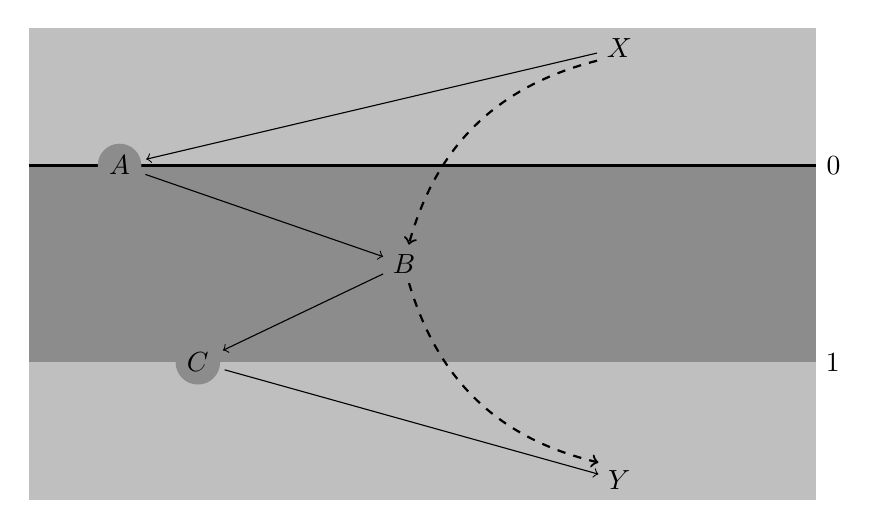
\begin{tikzpicture}
\begin{scope}
\clip (0,-3cm) rectangle (10,3cm);
\draw[line width=6cm,lightgray] (0,0) -- (10,0);
\draw[line width=2.5cm,gray!90!white] (0,0) -- (10,0);
\end{scope}
\draw[thick,yshift=1.25cm] (0,0) -- (10,0) node[right] {$0$};
\draw (10,-1.25) node[right] {$1$};
\node[above] (X) at (7.5,2.5) {$X$};
\node[below] (Y) at (7.5,-2.5) {$Y$};
\node[left,shape=circle,fill=gray!90!white,inner sep=.2em,outer sep=.2em]  (A) at (1.5,1.25) {$A$};
\node[right] (B) at (4.5,0) {$B$};
\node[left,shape=circle,fill=gray!90!white,inner sep=.2em,outer sep=.2em] (C) at (2.5,-1.25) {$C$};
\mor X f:r> Y;
\draw[->] (X) -- (A);
\draw[->] (A) -- (B);
\draw[->] (B) -- (C);
\draw[->] (C) -- (Y);
\draw[->,dashed,thick] (X.210) to [bend right] (B);
\draw[->,dashed,thick] (B) to [bend right] (Y.140);
\end{tikzpicture}
\caption{Tilting factorization of $f$.}
\label{tilting.fac}
\end{figure}
Even if the result can also be obtained from a direct argument, as a consequence of the following general fact about ternary FS:
\begin{lemma}[Tilting of factorizations]\label{tilted.FS}
Let $\tee\colon \Z\to \ts(\CC)$ be a $\Z$\hyp{}family of normal torsion theories on a stable $\infty$\hyp{}category $\CC$, having values $\tee_i = (\EE_i, \MM_i)$ for $i\in\Z$ (here, we will only consider the values $\tee_0, \tee_1 = \tee_0[1]$); let $(\LL,\mcal{R})$ be a torsion theory on the heart $\CC^\heart = \CC_{[0,1)}$ such that $\EE_1\subseteq \LL \subseteq \EE_0$ (equivalently, $\MM_0 \subseteq \R \subseteq \MM_1$). Then, the factorization $(e_{\tilt},m_{\tilt})$
\[
\begin{kD}
\lattice[mesh]{
\obj X; & \obj A; && \obj B; & \obj Y; \\
&& \obj S; &&\\	
};
\mor X e_1:-> A {e_0 \cdot m_1}:-> B m_0:-> Y;
\mor[swap] A l:-> S r:-> B;
\mor[dashed, L>,swap] X e_{\tilt}:-> S m_{\tilt}:-> Y;
\end{kD}
\]
of a morphism $f\colon X\to Y$ in $\CC$, obtained from the synergy of the ternary factorization induced by $\tee_0 \preceq \tee_1$ (see \refbf{multiple.fact}), plus the $(\mcal{L},\mcal{R})$\hyp{}factorization of its middle part $A\to B \in \EE_0\cap \MM_1$, defines a factorization system on $\CC$, called the \emph{tilting} of $\tee$ (confused with its $0$\hyp{}value $\tee_0$, in view of Remark \refbf{trivial.but.useful2}) by $(\LL, \R)$, and denoted $\tee\tilt (\LL,\R)$.
\end{lemma}
\begin{proof}
We have to show that the rule outlined above constitutes a factorization system; the stretagy is to summon \cite[\athm \textbf{A}]{Korostenski199357} again (see the proof of the ``Rosetta stone'' \refbf{thm:rosetta});
there is, however, also a direct proof of this fact, appealing the ``$\semicol$'' notation of \refbf{fat.notation}: it's easy to see that (in the notation of the statement) $\EE_1\perp \R\semicol\MM_0$ and $\LL\perp \R\semicol\MM_0$. Now, this allows us to conclude since given a lifting problem
\[
\begin{kD}
\lattice[mesh]{
\obj X; & \obj A; \\
\obj Y; & \obj B; \\	
\obj Z; & \obj C; \\
};
\mor X u:-> A r:-> B m_0:-> C;
\mor[swap] X e_1:-> Y l:-> Z v:-> C;
\mor[dashed] Y x:-> C;
\mor[dashed] Y y:-> A;
\mor[dashed] Z z:-> A;
\end{kD}
\]
the arrows $x,y,z$ obtained respectively as composition $v\circ l$, and as solutions to suitable lifting problems, give the desired orthogonality.
\end{proof}
\section{Algebras for a monad}
\index{T-algebras@$T$\hyp{}Algebras}
% \epigraph{MANCA!}{}
In the present section we sketch a general method to induce a $t$\hyp{}structure on the stable $\infty$\hyp{}category of algebras for a monad $T$ on a stable $\CC$. Apart from some locally\hyp{}defined new conventions, the same notation as in the rest of the text applies here. 
\begin{lemma}
Let $\fF=(\EE,\MM)$ be a factorization system on $\CC$ and $T$ a monad on $\CC$ that preserves the marking $\EE$ of $\fF$, \ie such that $T\EE\subset \EE$; then there is a factorization system $(\EE',\MM')=U^\leftarrow(\fF)$ on $\CC^T$ (the \textsc{em} category of algebras for the monad $T$) defined by $\EE' = U^\leftarrow(\EE), \MM' = U^\leftarrow(\MM)$.
\end{lemma}
\begin{proposition}
If $\CC$ is a stable $\infty$\hyp{}category and $T\colon \CC\to \CC$ a monad on $\CC$ which preserves finite colimits, then the category $\CC^T$ of $T$\hyp{}algebras is again stable.
\end{proposition}
\begin{proposition}[$t$\hyp{}structure on $T$\hyp{}algebras]
Given a $t$\hyp{}structure $\tee$ on $\CC$, whose normal torsion theory is $\fF=(\EE,\MM)$, the procedure above defines a $t$\hyp{}structure on the category of $T$\hyp{}algebras $\CC^T$, for $T$ a $\EE$\hyp{}preserving finitely cocontinuous monad on $\CC$.
\end{proposition}
\begin{proof}
To show that $U^\leftarrow(\fF)$ is a normal torsion theory we have to show that
\begin{enumerate}
\item $\fF'$ is bireflective, \ie both $\EE',\MM'$ are 3\hyp{}for\hyp{}2 classes;
\item $\fF'$ is normal \ie one of the equivalent conditions blabla is satisfied.
\end{enumerate}
The preimage of a 3\hyp{}for\hyp{}2 class under any functor is again 3\hyp{}for\hyp{}2. This proves the first item. Normality follows from the assumptions in the following form:
\begin{quote}
the arrow $(KX,k)\to 0$ lies in $\EE'$, for each $(X,x)\in \CC^T$, if we take $(KX, k)$ to be the fiber 
\[
\begin{kD}
\lattice[mesh={4em}{6em}]{
	\obj KX; & \obj (X):(X,x); \\
	\obj 0; & \obj (RX):(RX,r); \\
};
\mor KX -> X -> RX <- 0 <- KX;
\end{kD}
\]
of $(X,x)\to (RX,r)$ (the reflection associated to $\fF$).\qedhere
\end{quote}
\end{proof}
Application: let $\CC$ be stable and monoidal; any internal monoid $M$ in $\CC$ induces a monad $-\otimes M$; unders suitable assumptions, the category of $M$\hyp{}objects (algebras for $-\otimes M$) inherits a $t$\hyp{}structure.